\documentclass[preprint,12pt]{elsarticle}
%% Preamble as in the course template (Sample_Template), plus TikZ libraries for the diagrams.
\usepackage{lineno,hyperref}
\usepackage{booktabs}
\usepackage[english]{babel}
\usepackage[utf8]{inputenc}
\usepackage{amsfonts}
\usepackage{graphicx}
\usepackage{amssymb,amsmath}
\usepackage{float}
\usepackage{ragged2e}
\usepackage{adjustbox}
\usepackage{multicol}
\usepackage[justification=centering]{caption}
\usepackage{algorithm}
\usepackage{algpseudocode}
\usepackage{multirow}
\usepackage{mathtools}
\usepackage{color}
\usepackage{soul}
\usepackage{comment}
\usepackage{lscape}
\usepackage{setspace}
\doublespacing

\algnewcommand\algorithmicforeach{\textbf{for each}}
\algdef{S}[FOR]{ForEach}[1]{\algorithmicforeach\ #1\ \algorithmicdo}

\usepackage{tikz}
\usetikzlibrary{positioning,arrows.meta,fit,backgrounds,calc,shapes.geometric}
\def\checkmark{\tikz\fill[scale=0.3](0,.35) -- (.25,0) -- (1,.7) -- (.25,.15) -- cycle;}

\usepackage{array}
\newcolumntype{L}[1]{>{\raggedright\let\newline\\\arraybackslash\hspace{0pt}}m{#1}}
\newcolumntype{C}[1]{>{\centering\let\newline\\\arraybackslash\hspace{0pt}}m{#1}}
\newcolumntype{R}[1]{>{\raggedleft\let\newline\\\arraybackslash\hspace{0pt}}m{#1}}
\newcolumntype{P}[1]{>{\centering\arraybackslash}p{#1}}

\captionsetup{singlelinecheck=false, format=hang, justification=justified, font=footnotesize, labelsep=space}
\modulolinenumbers[5]
\journal{Elsevier}
\bibliographystyle{elsarticle-num}

%% Names used throughout
\newcommand{\vrroom}{\texttt{vr\_room}}
\newcommand{\captwo}{\texttt{cap2}}

\begin{document}

\begin{frontmatter}

\title{RoomRecon: Walkable Indoor Reconstruction from Smartphone Captures with Depth-Guided Gaussian Splatting, and an Evaluation of Walk-Collision Accuracy}

\author[1]{Aswin M\corref{cor1}\fnref{roll1}}
\author[1]{Sejal Satheesh\fnref{roll2}}
\cortext[cor1]{Corresponding author}
\fntext[roll1]{Roll No. 2023BCS0012}
\fntext[roll2]{Roll No. 2023BCS0048}
\address[1]{Indian Institute of Information Technology, Kottayam, India}

\begin{abstract}
A photoreal 3D copy of a room that a person can walk through needs a model that looks right from anywhere in the room and collision that stops the walker at the real walls. Gaussian splatting provides the first, but plain walls defeat camera poses estimated from images, and the walk collision that viewers build from a splat has not been checked against the real room. We present RoomRecon, which turns an iPhone capture (ARKit poses and LiDAR depth) into a first-person walkable model by reusing maintained tools (nerfstudio with DN-Splatter, splat-transform and the SuperSplat Viewer), and adds the glue they lack and an evaluation of walk collision against a laser scan. On the MuSHRoom \texttt{vr\_room} scene, DN-Splatter reached 26.3\,dB PSNR on held-out frames with a mesh 1.8\,cm from the laser scan (plain splats: 5.9\,cm); our own room reached 22.2\,dB, and both rooms were walkable on a laptop GPU. Collision built from DN-Splatter's mesh matched the scan's walkable area with an IoU of 0.81 and missed 1.7\% of the walls, against 0.58 and 17.8\% for the default collision built from the splat; Polycam's mesh scored 0.79 and 1.8\%. The mesh met three of our four pre-agreed criteria, although a free walk did not reveal the difference. Two other novelty attempts failed their pre-agreed tests and are reported as negative results.

\end{abstract}

\begin{highlights}
\item An iPhone room capture becomes a photoreal Gaussian splat you can walk through.
\item Built by reusing maintained tools; our code is the glue and the evaluation.
\item Collision from a depth-guided mesh fits a laser scan far better than from splats.
\item Two other novelty attempts failed their pre-agreed tests; both are reported.
\end{highlights}

\begin{keyword}
Gaussian splatting \sep Indoor reconstruction \sep Smartphone capture \sep LiDAR \sep Walk collision \sep Virtual walkthrough
\end{keyword}

\end{frontmatter}

\linenumbers
\section{Introduction}
\label{sec:intro}

A 3D copy of a real room that looks real and can be explored on foot is useful for visiting a place remotely, for planning changes to a space and for testing robots that move indoors \cite{chen2026neverwhere, liu2026navgsim}. Neural radiance fields \cite{mildenhall2020nerf} and 3D Gaussian splatting (3DGS) \cite{kerbl3dgs} reconstruct such copies from photographs, and 3DGS renders them in real time. Capture has become cheap: an iPhone records each frame with its own camera pose from ARKit, and the Pro models add a LiDAR depth map.

Getting from a phone capture to a room one can walk in still has two weak points. First, rooms are dominated by plain walls, ceilings and floors. Camera poses estimated from the images fail on such surfaces, and the trained model has little to constrain its geometry; DN-Splatter \cite{turkulainen2025dnsplatter} and later methods \cite{ren2025agsmesh, ruan2025indoorgs, jin2025planargs} add depth, normal or planar priors for this reason. Second, walking needs collision that stops the walker at the walls. The SuperSplat Viewer's walk mode \cite{supersplatwalk, supersplatviewer} builds it automatically from the splat with splat-transform \cite{splattransform}, but we found no measurement of how closely this collision follows the real walls.

Our first attempt (v1, August--September 2026) estimated poses from images and failed on a plain-walled bedroom (Section~\ref{sec:journey}). We restarted as RoomRecon v2 around one rule: reuse maintained tools and write only the glue between them. The phone supplies poses and depth, DN-Splatter on nerfstudio \cite{tancik2023nerfstudio} trains the model on a shared GPU, and splat-transform and the SuperSplat Viewer provide collision and walking on a laptop (Figure~\ref{fig:teaser}).

\begin{figure}[!htb]
	\centering
	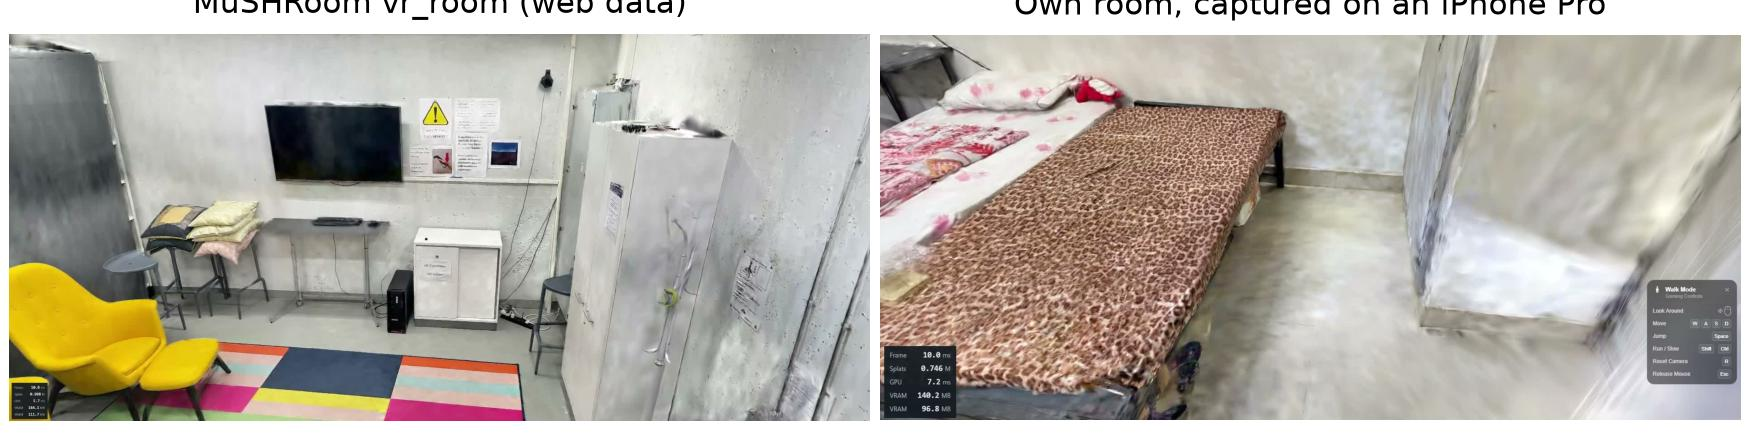
\includegraphics[width=\linewidth]{figures/teaser.jpg}
	\caption{First-person walk in the SuperSplat Viewer on a laptop (RTX~3050, 6\,GB), frames from our screen recordings. Left: MuSHRoom \texttt{vr\_room} (0.91\,M Gaussians). Right: our own room, captured on an iPhone~13~Pro (0.75\,M Gaussians). The lower-left overlay is the viewer's frame-time counter.}
	\label{fig:teaser}
\end{figure}

The salient contributions of this work are:
\begin{enumerate}
    \item \textbf{A working pipeline from an iPhone capture to a walkable Gaussian splat}, assembled from existing tools plus our glue (training settings for a shared GPU, automatic alignment of up direction, floor, scale and starting point, offline demo bundles), shown on a public room with a laser scan (MuSHRoom \texttt{vr\_room} \cite{ren2024mushroom}) and on our own room.
    \item \textbf{A measurement of walk-collision accuracy against a laser scan}, comparing collision built from DN-Splatter's mesh with the default built from the splat, with raw phone LiDAR and with Polycam's mesh, under criteria fixed before the run.
    \item \textbf{An account of what we explored and learned}, including the v1 failures that shaped v2 and two novelty attempts that failed their pre-agreed tests and are reported as negative results.
\end{enumerate}

The organisation of the report is as follows. Section~\ref{sec:related} discusses related work and its limitations. Section~\ref{sec:journey} describes how we explored the problem and what we learned. Section~\ref{sec:method} presents the pipeline and the collision evaluation. Section~\ref{sec:results} gives the datasets, setup and results, including a comparison with existing implementations. Section~\ref{sec:conclusion} concludes with two directions for future work.

\section{Related works}
\label{sec:related}

This section discusses the work our pipeline builds on and is measured against, grouped by the question each line of work answers. For each work we give the problem, the method and the outcome reported by its authors.

\subsection{Radiance fields and splatting toolkits}
NeRF \cite{mildenhall2020nerf} represents a scene as a neural field rendered by volume rendering; 3DGS \cite{kerbl3dgs} replaces it with millions of anisotropic Gaussians rasterised in real time. Nerfstudio \cite{tancik2023nerfstudio} is a modular framework for such methods, with data importers, a viewer and export tools, and its rasteriser library gsplat \cite{ye2025gsplat} reports up to 10\% less training time and 4$\times$ less memory than the original 3DGS code. 2D Gaussian splatting \cite{huang2024twodgs} improves the poor surfaces of 3DGS by collapsing the Gaussians into oriented disks with depth-distortion and normal-consistency terms, and reports detailed, noise-free geometry. 3DGS-MCMC \cite{kheradmand2024mcmc}, used in our v1, recasts densification as Markov chain Monte Carlo sampling.

\subsection{Gaussian splatting for indoor rooms}
DN-Splatter \cite{turkulainen2025dnsplatter} targets textureless indoor scenes: it supervises the Gaussians with sensor depth through a loss weighted by image gradients, adds a smoothness term and monocular normals, and extracts a mesh directly from the result. AGS-Mesh \cite{ren2025agsmesh} notes that phone depth is coarse and monocular normals are inconsistent across views, filters these priors by their consistency during training and adds a scale-aware meshing step, improving meshes and novel views on indoor room datasets. GaussianRoom \cite{xiang2025gaussianroom} couples a neural signed distance field with 3DGS to guide densification and pruning, with normal and edge priors for textureless areas, and reports state-of-the-art results on ScanNet and ScanNet++. IndoorGS \cite{ruan2025indoorgs} lifts 2D line segments to 3D and derives plane cues for textureless regions to drive initialisation and density control, reporting more accurate geometry and rendering. PlanarGS \cite{jin2025planargs} finds planar regions with a vision-language segmentation model and supervises the Gaussians with planar and depth/normal terms, outperforming earlier methods on indoor benchmarks. LighthouseGS \cite{han2026lighthousegs} handles panorama-style phone captures by using the phone's poses and monocular depth as rough priors, initialising on planes and correcting drift and auto-exposure. PocketGS \cite{guo2026pocketgs} trains 3DGS on the phone itself within minutes. All of these report image quality and surface accuracy; none asks whether a person can walk in the result.

\subsection{Camera poses from images alone}
COLMAP \cite{schoenberger2016colmap} recovers poses by matching local features; learned features such as SuperPoint \cite{detone2018superpoint} with LightGlue \cite{lindenberger2023lightglue} in hloc \cite{sarlin2019hloc}, and visual SLAM such as ORB-SLAM3 \cite{campos2021orbslam3}, rely on the same principle. MASt3R-SfM \cite{duisterhof2025mast3rsfm} builds structure from motion on a 3D foundation model and aligns its local reconstructions at linear cost; VGGT \cite{wang2025vggt} predicts cameras, depth and point maps from up to hundreds of views in one forward pass, in under a second. These newer models depend less on texture than the methods that failed in our v1, but we did not test them; taking poses from the phone removed the problem for this project.

\subsection{Walking and navigating in Gaussian splats}
The SuperSplat Viewer \cite{supersplatviewer} offers a first-person walk mode whose collision is a voxel volume generated from the splat by splat-transform \cite{splattransform, supersplatwalk}. Splat-Nav \cite{chen2025splatnav} plans safe robot trajectories directly in a splat map using collision constraints derived from the Gaussians, tested in 126 hardware flights. NavGSim \cite{liu2026navgsim} is a splat-based simulator for multi-room navigation that extracts navigable areas by slicing the Gaussians. The Neverwhere benchmark \cite{chen2026neverwhere} turns more than sixty splat reconstructions into closed-loop tests for visual legged locomotion, and LucidSim \cite{yu2024lucidsim} trains a visual parkour policy from generated images; in both, physics runs on separate collision geometry while the images come from the splat or a generator. None of these reports how accurately its collision follows the real walls.

\subsection{Capture guidance and view selection}
Kopanas and Drettakis \cite{kopanas2023placement} place cameras for free-viewpoint navigation in rooms using observation frequency and angular uniformity. FisherRF \cite{jiang2024fisherrf} picks the next view by expected information gain from the Fisher information of the model's parameters, while NeRF Director \cite{xiao2024nerfdirector} shows that uniform coverage alone, without any uncertainty estimate, selects good training views. COVER \cite{chen2026cover} shows that an approximation of the Fisher information gain reduces to covering geometry that past cameras saw poorly, and AGILE-GS \cite{khass2026agilegs} cuts next-best-view selection time by one to two orders of magnitude. For people capturing with phones, Zhang et al.\ \cite{zhang2026objectcentered} guide object captures live by spherical coverage and beat free capture with fewer images; Yasunaga et al.\ \cite{yasunaga2025userloop} show in augmented reality where a quick reconstruction is wrong so that the user adds views there; LiMRSF \cite{chang2026limrsf} overlays a LiDAR SLAM point cloud on the real room in a mixed-reality headset to reveal blind spots and double walls while scanning. MUGSQA \cite{chen2026mugsqa} collects human quality ratings of splats reconstructed from inputs of varying number, resolution and viewing distance.

\subsection{Limitations of existing work}
Limitations of the existing methods, as they affect a walkable room, are:
\begin{itemize}
    \item Indoor splatting methods are evaluated on image and mesh quality only; walkability is not tested.
    \item Walk collision built from a splat is the default in a widely used viewer, but its accuracy against a ground-truth scan is not published; robotics work pairs splats with separate collision geometry without measuring the difference.
    \item Pose estimation from images alone still struggles in plain-walled rooms (our v1; the newest feed-forward models were not tested).
    \item Capture feedback is live, object-scale, or needs special hardware or a trained model; none checks an exported room capture before training.
    \item The path from a phone to a walkable room spans separate tools with different coordinate conventions and defaults that do not suit a shared GPU.
\end{itemize}
We address the first, second and last points directly (Sections~\ref{sec:method} and~\ref{sec:collision-results}). The fourth was our first novelty attempt, which failed its own test (Section~\ref{sec:negative}); the third is future work.

\section{What we explored and learned}
\label{sec:journey}

The pipeline of Section~\ref{sec:method} is the result of two attempts, several failures and a few measurements that changed our plans (Figure~\ref{fig:journey}). This section follows them in order, because most of what we learned came from them.

\begin{figure}[!htb]
\centering
\begin{adjustbox}{max width=\linewidth}
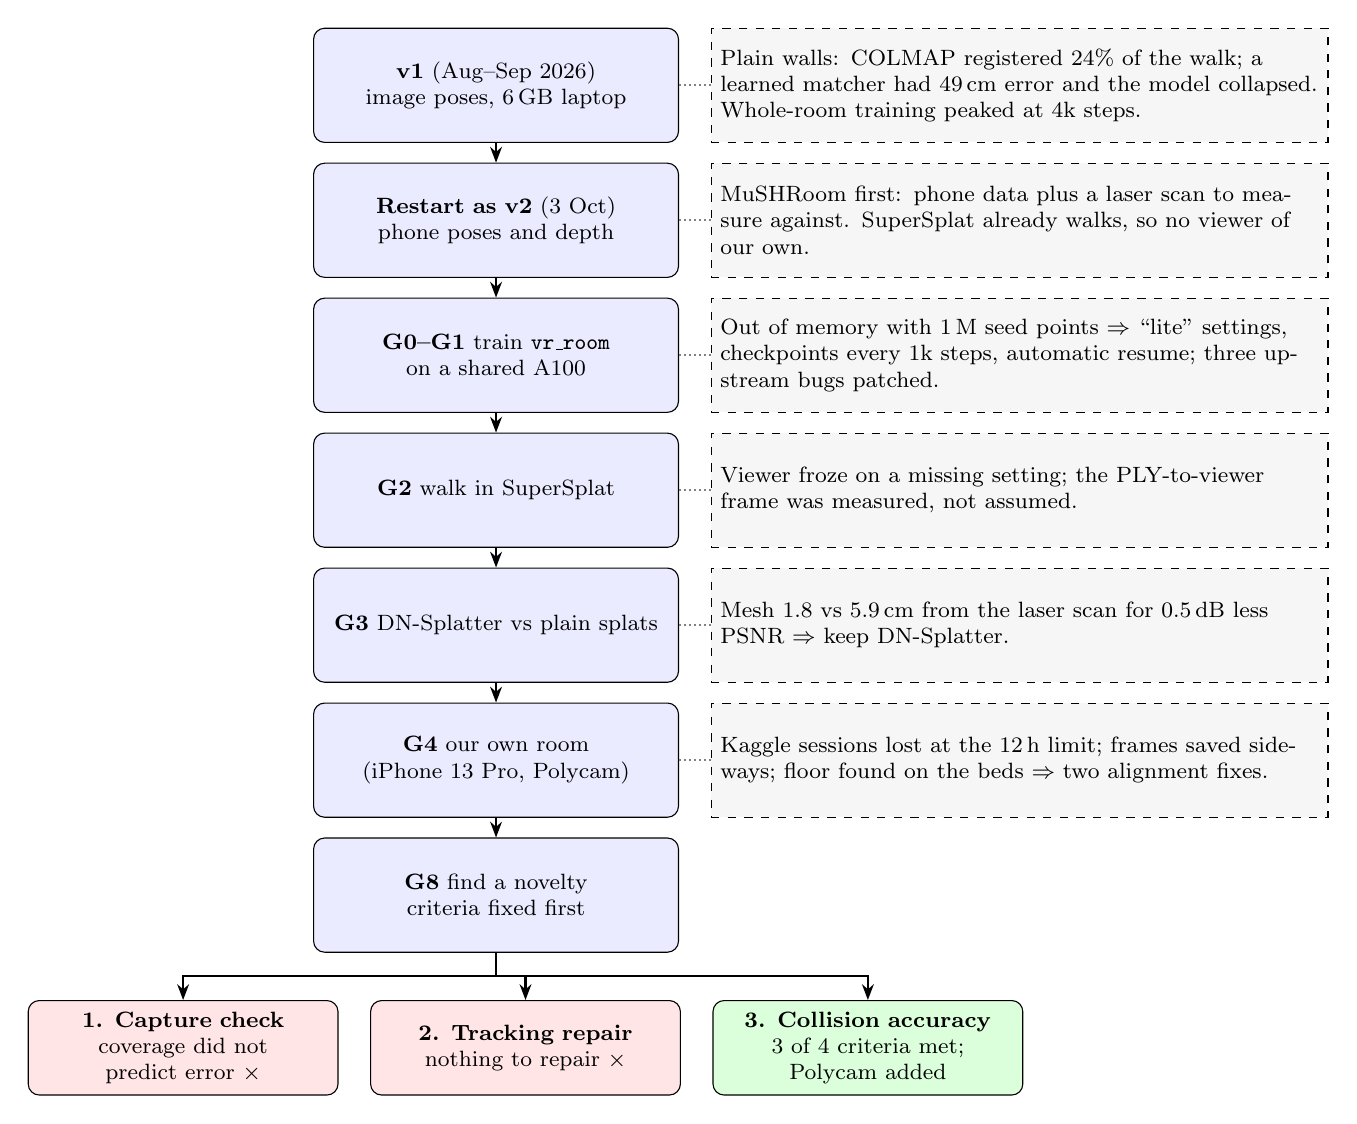
\begin{tikzpicture}[
  node distance=2.5mm and 4mm,
  every node/.style={font=\footnotesize\setstretch{1}},
  phase/.style={draw, rounded corners, fill=blue!8, text width=4.4cm, align=center, minimum height=14.5mm},
  note/.style={draw, dashed, fill=gray!7, text width=7.6cm, align=left, minimum height=14.5mm},
  bad/.style={draw, rounded corners, fill=red!10, text width=3.7cm, align=center, minimum height=12mm},
  good/.style={draw, rounded corners, fill=green!14, text width=3.7cm, align=center, minimum height=12mm},
  arr/.style={-{Stealth[length=2mm]}, thick},
  lnk/.style={densely dotted, thick, gray}]
\node[phase] (v1) {\textbf{v1} (Aug--Sep 2026)\\image poses, 6\,GB laptop};
\node[note, right=of v1] (n1) {Plain walls: COLMAP registered 24\% of the walk; a learned matcher had 49\,cm error and the model collapsed. Whole-room training peaked at 4k steps.};
\node[phase, below=of v1] (re) {\textbf{Restart as v2} (3 Oct)\\phone poses and depth};
\node[note, right=of re] (n2) {MuSHRoom first: phone data plus a laser scan to measure against. SuperSplat already walks, so no viewer of our own.};
\node[phase, below=of re] (g1) {\textbf{G0--G1} train \texttt{vr\_room}\\on a shared A100};
\node[note, right=of g1] (n3) {Out of memory with 1\,M seed points $\Rightarrow$ ``lite'' settings, checkpoints every 1k steps, automatic resume; three upstream bugs patched.};
\node[phase, below=of g1] (g2) {\textbf{G2} walk in SuperSplat};
\node[note, right=of g2] (n4) {Viewer froze on a missing setting; the PLY-to-viewer frame was measured, not assumed.};
\node[phase, below=of g2] (g3) {\textbf{G3} DN-Splatter vs plain splats};
\node[note, right=of g3] (n5) {Mesh 1.8 vs 5.9\,cm from the laser scan for 0.5\,dB less PSNR $\Rightarrow$ keep DN-Splatter.};
\node[phase, below=of g3] (g4) {\textbf{G4} our own room\\(iPhone 13 Pro, Polycam)};
\node[note, right=of g4] (n6) {Kaggle sessions lost at the 12\,h limit; frames saved sideways; floor found on the beds $\Rightarrow$ two alignment fixes.};
\node[phase, below=of g4] (g8) {\textbf{G8} find a novelty\\criteria fixed first};
\node[bad, below=6mm of g8.south, xshift=-2.0cm, anchor=north east] (a1) {\textbf{1. Capture check}\\coverage did not predict error $\times$};
\node[bad, right=4mm of a1] (a2) {\textbf{2. Tracking repair}\\nothing to repair $\times$};
\node[good, right=4mm of a2] (a3) {\textbf{3. Collision accuracy}\\3 of 4 criteria met; Polycam added};
\foreach \a/\b in {v1/re, re/g1, g1/g2, g2/g3, g3/g4, g4/g8} \draw[arr] (\a) -- (\b);
\foreach \a/\b in {v1/n1, re/n2, g1/n3, g2/n4, g3/n5, g4/n6} \draw[lnk] (\a) -- (\b);
\draw[arr] (g8.south) -- ++(0,-3mm) -| (a1.north);
\draw[arr] (g8.south) -- ++(0,-3mm) -| (a2.north);
\draw[arr] (g8.south) -- ++(0,-3mm) -| (a3.north);
\end{tikzpicture}
\end{adjustbox}
\caption{How the project developed. Blue: goals worked through in order; dashed: what each step taught us; red and green: the three novelty attempts and whether they met the criteria fixed before running them.}
\label{fig:journey}
\end{figure}

\subsection{v1: poses from images on a laptop}
Our first version aimed to reconstruct a room from RGB images alone and to train on a laptop (RTX~3050, 6\,GB). The test room was a plain-walled ARKitScenes \cite{baruch2021arkitscenes} bedroom (scene 41254269, a 95\,s iPad walk). Table~\ref{tab:v1poses} compares the pose sources we tried against the iPad's own ARKit poses. COLMAP \cite{schoenberger2016colmap} was accurate but registered only a quarter of the walk; SuperPoint \cite{detone2018superpoint} and LightGlue \cite{lindenberger2023lightglue} in hloc \cite{sarlin2019hloc} registered every frame with 49\,cm error, and 3DGS trained on those poses rendered every view as flat colour. A textured utility room, by contrast, tracked cleanly (COLMAP: all frames, 1.6\,cm). Image-only poses failed specifically on plain walls, and accuracy mattered more than coverage.

\begin{table}[!htb]
\caption{v1 pose sources on the plain-walled ARKitScenes bedroom 41254269 (laptop). Error is measured against the iPad's ARKit poses.}
\label{tab:v1poses}
\centering
\begin{tabular}{lccl}
\hline
\textbf{Pose source} & \textbf{Walk covered} & \textbf{Error} & \textbf{3DGS result} \\
\hline
COLMAP, SIFT & 24\% & 1.2\,cm & sharp, a quarter of the room \\
SuperPoint + LightGlue & 100\% & 49\,cm & total collapse \\
ORB-SLAM3 \cite{campos2021orbslam3}, mono & 7--93\% & 6--52\,cm & not trained (4--6 maps) \\
ARKit device poses & 100\% & reference & see Figure~\ref{fig:curves} \\
\hline
\end{tabular}
\end{table}

Even with ARKit poses, whole-room training did not hold: a 22\,s window of the walk reached 30.3\,dB on held-out frames, but the full walk peaked at 22.8\,dB after 4,000 steps and fell to 13.7\,dB by 15,000 (Figure~\ref{fig:curves}, left). Switching densification from MCMC \cite{kheradmand2024mcmc} to the default only slowed the decline, and we never found the cause. Only evaluating every 1,000 steps revealed the early peak; the final number alone said ``failure''. v1 also showed that its browser viewer, GaussianSplats3D \cite{gaussiansplats3d}, dropped to 8 frames per second (95th percentile) at a million Gaussians, and that a 32-photo phone capture made with NeRFCapture \cite{nerfcapture} trained to only 16.0\,dB, full of streaks and floaters.

\begin{figure}[!htb]
	\centering
	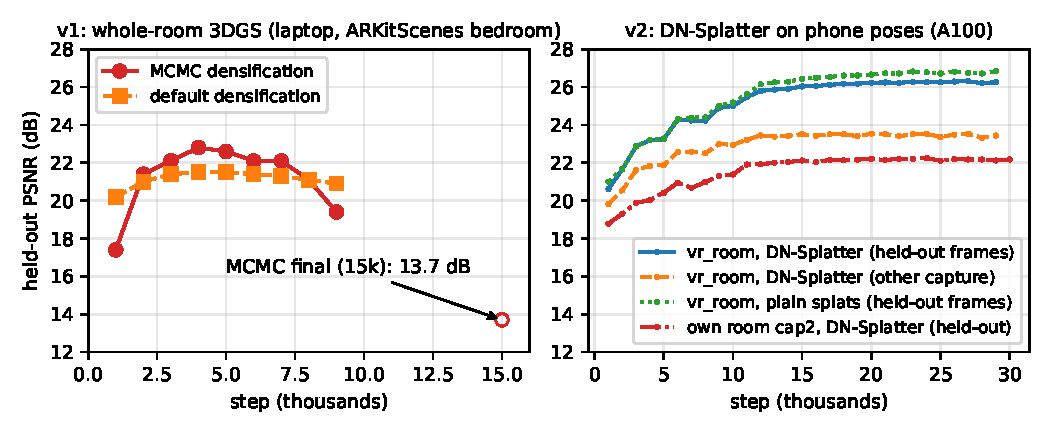
\includegraphics[width=\linewidth]{figures/curves.pdf}
	\caption{Held-out PSNR during training, evaluated every 1,000 steps. Left: v1, the full bedroom walk with ARKit poses on the laptop (from our v1 log; after 9k only the final value at 15k was recorded). Right: v2 on the A100: DN-Splatter on \texttt{vr\_room} (held-out frames of the training walk and frames of a separate walk), plain splats on the same data, and our own room. No v2 run collapsed.}
	\label{fig:curves}
\end{figure}

\subsection{Restarting as v2}
We kept the goal and changed the approach. The phone tracks its own pose by combining the camera with its inertial sensors, and those poses had trained a usable model where image-only poses had not, so v2 takes poses (and LiDAR depth) from the phone. DN-Splatter was chosen because it targets plain indoor surfaces and ships a loader for MuSHRoom, whose rooms come with iPhone data and a laser scan. SuperSplat already offered first-person walking with collision, so our plan to build a viewer in Unity was dropped. Training moved to a campus A100, and the work was organised as goals in priority order, each with exit criteria, so that unfinished goals could be cut from the end.

\subsection{Research code on a shared GPU}
Another user held 33--35\,GB of the A100's 40\,GB. DN-Splatter seeds one million Gaussians by default, and our first full run ran out of memory at about step 1,000. We changed as little as possible: 300k seed points, splitting stopped at step 10,000 instead of 15,000, and a wrapper that resumes from the newest checkpoint after a crash; a deliberate kill-and-resume test continued at step 1,001. Three upstream bugs had to be patched (an evaluation key error, a crash on resuming with an empty optimiser state, and resumed runs repeating their full step count), and the environment needed pins against conflicting dependency versions. Research code assumes a dedicated GPU and one uninterrupted run; checkpoints, regular evaluation and automatic resume are what made our runs finish.

\subsection{From a trained model to a walkable room}
A trained splat has no notion of up, floor, size or starting point. The viewer loads a PLY rotated by 180$^\circ$ about $z$, and its Euler-angle convention is undocumented; we measured both rather than assume them. The first walk test failed because our settings file lacked a block the viewer's newer schema requires. Our own room then broke two assumptions of our alignment. Polycam had saved every frame sideways, so the cameras' mean up vector averaged to almost nothing; up is now taken from the camera's $-x$ axis when $+y$ disagrees. The floor had been taken as the densest level below the cameras, which here was the tops of the beds, and the room came out 1.68 times too large; the floor is now the lowest dense level (Algorithm~\ref{alg:scene}). Against MuSHRoom's laser scan, the old rule had put the \texttt{vr\_room} floor 13\,cm too high and the new one is within about 1.5\,cm. The released \texttt{vr\_room} demo predates this fix and was deliberately kept as walk-tested.

\subsection{Capturing our own room}
Sejal captured a bedroom three times on an iPhone~13~Pro with Polycam's raw-data export \cite{polycam}. The first capture (32 frames) was too sparse, as v1 had predicted; the second (257 frames, one tracking segment) covered the room and was used; the third (491 frames) had three tracking segments with pose jumps of about 2\,m. While the A100 was full we tried Kaggle's free GPUs, but both sessions ran to Kaggle's 12-hour limit without saving output, most likely because our memory sampler outlived the training script (now stopped explicitly). Back on the A100, the run crashed once at step 10,400, resumed by itself from step 10,000 and finished.

\subsection{Looking for a novelty}
For each novelty idea we searched the literature first and fixed pass/fail criteria in writing before running anything. A capture check before training (Section~\ref{sec:capcheck-method}) failed its validation; a repair of \texttt{cap3}'s broken tracking found nothing to repair; the accuracy of walk collision met three of four criteria and is the result we lead with (Section~\ref{sec:results}).

The lessons that shaped the final design:
\begin{itemize}
\item take poses from the phone, since image-only poses failed on plain walls;
\item evaluate every 1,000 steps and look at renders, since a final number alone hid a collapse;
\item measure coordinate conventions and check alignment against a scan, since two of our assumptions were wrong on real data;
\item assume the GPU will run out: checkpoint, resume and keep evidence off the machine;
\item fix success criteria before the run and report the outcome either way.
\end{itemize}

\section{Proposed method}
\label{sec:method}

RoomRecon turns a phone capture into a Gaussian splat that can be walked through with collision, and measures how accurate that collision is. Almost every stage is an existing program; our code connects the stages, adapts their defaults and adds the alignment and evaluation steps that do not exist elsewhere (Figure~\ref{fig:arch}).

\begin{figure}[!htb]
\centering
\begin{adjustbox}{max width=\linewidth}
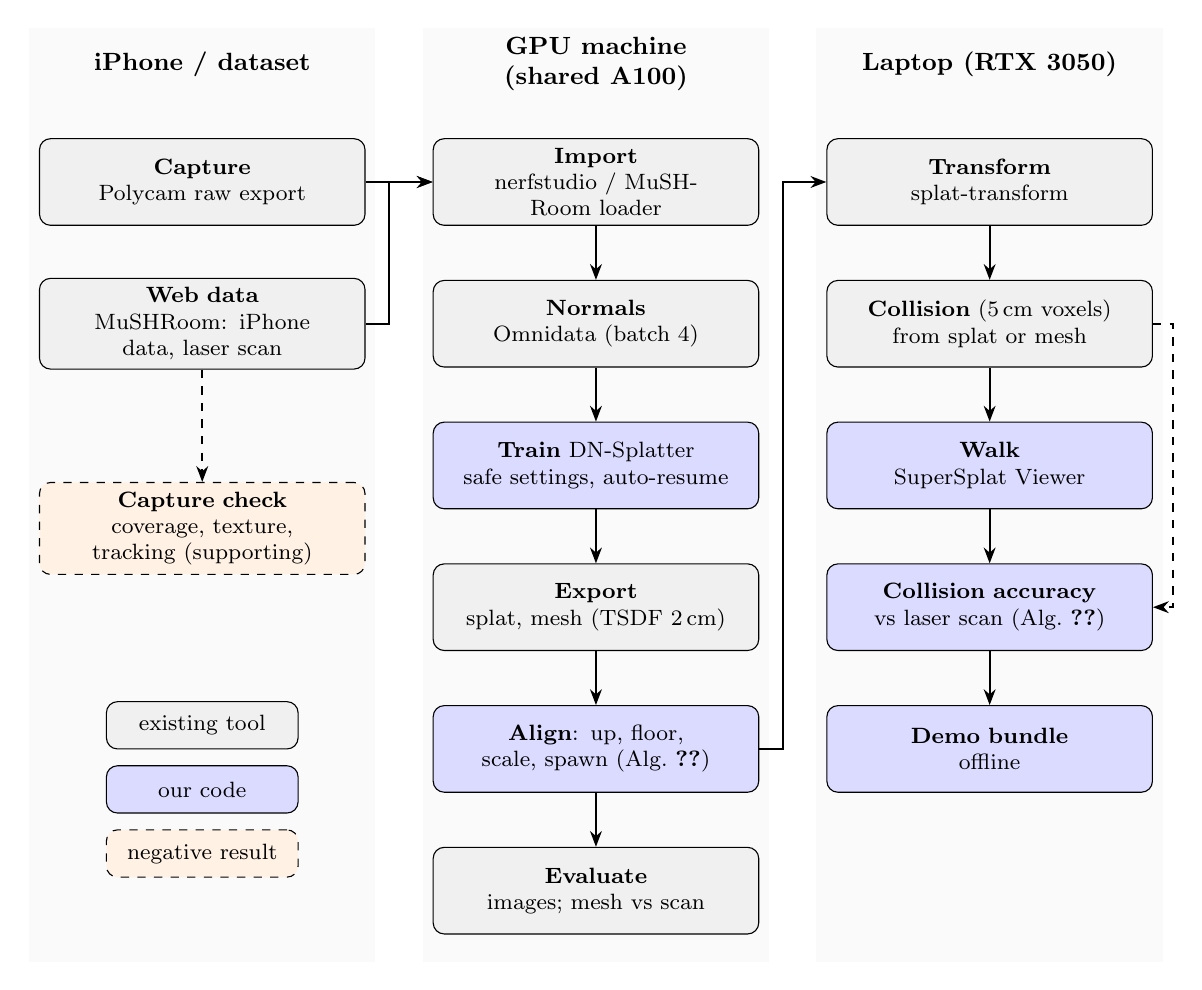
\begin{tikzpicture}[
  every node/.style={font=\footnotesize\setstretch{1}},
  tool/.style={draw, rounded corners, fill=gray!12, text width=3.9cm, align=center, minimum height=11mm},
  ours/.style={draw, rounded corners, fill=blue!14, text width=3.9cm, align=center, minimum height=11mm},
  side/.style={draw, rounded corners, dashed, fill=orange!10, text width=3.9cm, align=center, minimum height=11mm},
  lane/.style={font=\small\bfseries\setstretch{1}, text width=4.2cm, align=center},
  arr/.style={-{Stealth[length=2mm]}, thick},
  opt/.style={-{Stealth[length=2mm]}, thick, dashed}]
\node[lane] at (0,0) {iPhone / dataset};
\node[lane] at (5.0,0) {GPU machine (shared A100)};
\node[lane] at (10.0,0) {Laptop (RTX 3050)};
\node[tool] (cap) at (0,-1.5) {\textbf{Capture}\\Polycam raw export};
\node[tool] (mush) at (0,-3.3) {\textbf{Web data}\\MuSHRoom: iPhone data, laser scan};
\node[side] (cc) at (0,-5.9) {\textbf{Capture check}\\coverage, texture, tracking (supporting)};
\node[tool] (imp) at (5.0,-1.5) {\textbf{Import}\\nerfstudio / MuSHRoom loader};
\node[tool] (nrm) at (5.0,-3.3) {\textbf{Normals}\\Omnidata (batch 4)};
\node[ours] (trn) at (5.0,-5.1) {\textbf{Train} DN-Splatter\\safe settings, auto-resume};
\node[tool] (exp) at (5.0,-6.9) {\textbf{Export}\\splat, mesh (TSDF 2\,cm)};
\node[ours] (aln) at (5.0,-8.7) {\textbf{Align}: up, floor,\\scale, spawn (Alg.~\ref{alg:scene})};
\node[tool] (evl) at (5.0,-10.5) {\textbf{Evaluate}\\images; mesh vs scan};
\node[tool] (rot) at (10.0,-1.5) {\textbf{Transform}\\splat-transform};
\node[tool] (col) at (10.0,-3.3) {\textbf{Collision} (5\,cm voxels)\\from splat or mesh};
\node[ours] (walk) at (10.0,-5.1) {\textbf{Walk}\\SuperSplat Viewer};
\node[ours] (acc) at (10.0,-6.9) {\textbf{Collision accuracy}\\vs laser scan (Alg.~\ref{alg:collision})};
\node[ours] (dem) at (10.0,-8.7) {\textbf{Demo bundle}\\offline};
\draw[arr] (cap) -- (imp);
\draw[arr] (mush.east) -- ++(0.3,0) |- (imp.west);
\draw[opt] (mush) -- (cc);
\draw[arr] (imp) -- (nrm);
\draw[arr] (nrm) -- (trn);
\draw[arr] (trn) -- (exp);
\draw[arr] (exp) -- (aln);
\draw[arr] (aln) -- (evl);
\draw[arr] (aln.east) -- ++(0.3,0) |- (rot.west);
\draw[arr] (rot) -- (col);
\draw[arr] (col) -- (walk);
\draw[opt] (col.east) -- ++(0.25,0) |- (acc.east);
\draw[arr] (walk) -- (acc);
\draw[arr] (acc) -- (dem);
\node[tool, text width=2.2cm, minimum height=6mm] (lg1) at (0,-8.4) {existing tool};
\node[ours, text width=2.2cm, minimum height=6mm, below=2mm of lg1] (lg2) {our code};
\node[side, text width=2.2cm, minimum height=6mm, below=2mm of lg2] {negative result};
\begin{scope}[on background layer]
\foreach \x in {0,5.0,10.0} \fill[gray!4] (\x-2.2,0.45) rectangle (\x+2.2,-11.4);
\end{scope}
\end{tikzpicture}
\end{adjustbox}
\caption{Architecture of RoomRecon. Grey: existing tools, used as they are or with small patches; blue: boxes containing our code (configuration, alignment, evaluation, packaging); orange: the supporting capture check, which failed its validation. Heavy work runs on the shared GPU machine; the laptop builds collision, shows the walk and runs the collision evaluation.}
\label{fig:arch}
\end{figure}

\subsection{Capture and import}
Own rooms are captured with Polycam's raw-data export \cite{polycam} on an iPhone with LiDAR: images, ARKit poses and intrinsics, a depth and confidence map per frame, and per-frame tracking data. nerfstudio's \texttt{ns-process-data polycam -{}-use-depth} converts it into a dataset; for MuSHRoom, DN-Splatter's own loader is used. Normals for the normal prior come from Omnidata \cite{eftekhar2021omnidata} through DN-Splatter's script, run in batches of four because the default batch does not fit beside the other GPU user. The initial Gaussians are 300,000 points back-projected from the LiDAR depth.

\subsection{Training with settings that suit a shared GPU}
\label{sec:training}
DN-Splatter \cite{turkulainen2025dnsplatter} adds three terms to the photometric loss of 3DGS: a depth loss against the LiDAR depth, weighted by image gradients so that edges are trusted less; a depth-smoothness term; and a loss against the monocular normals. We train for 30,000 steps with the changes in Table~\ref{tab:settings}. Besides memory, the pose setting matters: nerfstudio re-centres and re-scales poses by default, which would make the exports non-metric, while the phone's poses are already metric.

\begin{table}[!htb]
\caption{Training settings changed from the DN-Splatter / nerfstudio defaults. The two ``lite'' changes may cost quality; that cost was not measured.}
\label{tab:settings}
\centering
\small
\begin{tabular}{L{3.0cm}L{2.5cm}L{2.7cm}L{3.6cm}}
\hline
\textbf{Setting} & \textbf{Default} & \textbf{Ours} & \textbf{Why} \\
\hline
Seed points (lite) & 1,000,000 & 300,000 & out of memory with 5--7\,GB free \\
Stop splitting (lite) & step 15,000 & step 10,000 & caps the peak number of Gaussians \\
Checkpoints & only at the end & every 1k, keep all & a crash must not cost the run \\
Evaluation & effectively off & every 1k, all test images & a final-only metric hid a collapse \\
Pose processing & re-centre, re-scale & none (own data) & keep metric phone poses \\
Image cache & GPU & CPU & GPU memory \\
After a crash & manual restart & automatic resume & shared GPU \\
\hline
\end{tabular}
\end{table}

\subsection{Export and scene alignment}
The model is exported as a standard 3DGS PLY file and as a mesh, extracted by DN-Splatter with Open3D's TSDF fusion \cite{zhou2018open3d} at 2\,cm voxels. Neither file says which way is up, where the floor is, how large the room is or where to start. Algorithm~\ref{alg:scene} computes these from the cameras and the mesh, using two facts about handheld capture: the phone is held roughly upright, so the cameras' mean up vector gives gravity; and it is held near eye height, so the median camera height above the floor gives the scale. A scale near 1 confirms that the phone's poses were metric (1.038 for both of our rooms).

\begin{algorithm}[!htb]
	\caption{Scene alignment (\texttt{scene.json})}
	\label{alg:scene}
	\begin{algorithmic}[1]
		\Procedure{SceneFrame}{camera-to-world poses $\{T_i\}$, mesh vertices $V$}
		\State $u \gets$ mean of the cameras' $+y$ axes; \textbf{if} $\lVert u\rVert < 0.5$ \textbf{then} $u \gets$ mean of $-x$ axes
		\State \textbf{if} $\lVert u\rVert < 0.5$ \textbf{then fail} ``cannot estimate up''
		\State rotate camera centres $c_i$ and $V$ by $R$, which takes $u/\lVert u\rVert$ to $+y$
		\State $H \gets$ histogram (2\,cm bins) of vertex heights below the lowest camera
		\State $y_f \gets$ centre of the lowest local peak of $H$ holding $\ge 0.3 \max H$ \Comment{not the bed tops}
		\State $s \gets 1.45\,\mathrm{m} \,/\, \operatorname{median}_i (c_{i,y} - y_f)$ \Comment{eye height}
		\State $k \gets \arg\min_i \lVert c_i - \operatorname{median}_j c_j\rVert$ \Comment{a camera position is free space}
		\State spawn $\gets s\,c_k$ at height $s\,y_f + 1.45$\,m, facing camera $k$'s horizontal view
		\State \Return $R$ (as Euler angles in the viewer's frame), $s$, floor $s\,y_f$, spawn
		\EndProcedure
	\end{algorithmic}
\end{algorithm}

\subsection{Collision and walking}
On the laptop, splat-transform \cite{splattransform} applies the rotation and scale and builds the collision: it keeps the cluster of Gaussians connected to the spawn, voxelises it at 5\,cm (solid above an opacity of 0.1), fills the space outside the room, carves the space reachable from the spawn by a capsule 1.6\,m tall with a 0.2\,m radius, and writes a collision mesh. The SuperSplat Viewer \cite{supersplatviewer} 1.37.0 loads the splat, the collision and a settings file that places the start camera at the spawn, and its walk mode gives first-person movement. We patched only its interface size. For a demo independent of the network and the GPU machine, a script packs the viewer and the room into one folder.

\subsection{Evaluating walk-collision accuracy}
\label{sec:collision-method}
Our main measurement compares collision from DN-Splatter's mesh with the default collision from the splat, on \texttt{vr\_room}, which has a laser scan. Five sources go through exactly the demo's splat-transform pipeline, with the same rotation, scale and spawn:
\textbf{S}, the trained splat (the default, used in our demo);
\textbf{M}, points sampled every centimetre on DN-Splatter's mesh;
\textbf{L}, the raw phone LiDAR (depth maps back-projected into 3\,cm voxels, no training);
\textbf{P}, Polycam's own mesh of the same capture, shipped with MuSHRoom and aligned to the scan by ICP from 24 starting orientations (a best case for Polycam); and
\textbf{GT}, points on the laser scan, moved into the model's frame with MuSHRoom's alignment.
M, L, P and GT are written as small opaque splats (2\,cm) so that splat-transform treats them like a trained splat.

Each collision mesh is reduced to what matters for a walking person. Let $O_X$ be the 5\,cm floor-plan cells that contain collision surface between 0.2 and 1.8\,m above the floor, $W_X$ the free cells reachable from the spawn by four-connected steps, $d(c, O)$ the distance from cell $c$ to the nearest cell of $O$, and $\mathcal{S}$ the GT-occupied cells that the phone's LiDAR also saw (within 10\,cm). The measures are
\begin{align}
\mathrm{IoU}_X &= \frac{|W_X \cap W_{GT}|}{|W_X \cup W_{GT}|}, &
\mathrm{Phantom}_X &= A\{c \in O_X \cap W_{GT} : d(c, O_{GT}) > 10\,\mathrm{cm}\}, \\
\mathrm{Missed}_X &= \frac{|\{g \in \mathcal{S} : d(g, O_X) > 10\,\mathrm{cm}\}|}{|\mathcal{S}|}, &
\mathrm{Offset}_X &= \{d(c, O_{GT}) : c \in O_X,\ d(c, O_{GT}) \le 50\,\mathrm{cm}\},
\end{align}
where $A$ is area and the offset is summarised by its median and 95th percentile. A phantom obstacle blocks a place where the real room is free; a missed wall lets the walker through a real wall.

\begin{algorithm}[!htb]
	\caption{Walk-collision accuracy against a laser scan}
	\label{alg:collision}
	\begin{algorithmic}[1]
		\Procedure{CollisionAccuracy}{collision meshes $C_X$, scan and LiDAR points, \texttt{scene.json}}
		\State align the points with \texttt{scene.json}; $y_f \gets$ floor of the scan (Alg.~\ref{alg:scene}, line 6)
		\State grid $\gets$ 5\,cm cells over the scan's floor plan plus a 0.5\,m margin
		\ForEach{source $X \in \{S, M, L, P, GT\}$}
			\State sample $C_X$ every 1\,cm; $O_X \gets$ cells with samples at $0.2 \le y - y_f \le 1.8$\,m
			\State $W_X \gets$ flood fill from the spawn cell through cells not in $O_X$
		\EndFor
		\State compute Eqs.~(1)--(2) for each $X$ against GT; \textbf{pass} if M beats S on P1--P4
		\EndProcedure
	\end{algorithmic}
\end{algorithm}

The criteria, fixed before any run, were: P1, $\mathrm{IoU}_M \ge \mathrm{IoU}_S + 0.02$; P2, $\mathrm{Phantom}_M \le \mathrm{Phantom}_S$; P3, $\mathrm{Missed}_M \le \mathrm{Missed}_S + 2$ percentage points; P4, median $\mathrm{Offset}_M \le$ median $\mathrm{Offset}_S$.

\subsection{Capture check (supporting)}
\label{sec:capcheck-method}
The capture check runs right after a capture, before training, on what the phone recorded. It merges every frame's LiDAR depth (high-confidence pixels) into 3\,cm surface voxels, finds the frames that see each surface point by comparing its projection with each frame's own depth (so hidden walls do not count), and labels each point \textbf{under-covered} if fewer than 5 frames see it (the overlap that Pix4D's photogrammetry quality reports treat as sufficient) or its viewing directions fill fewer than 3 of 64 direction bins (COVER's angular coverage \cite{chen2026cover}, moved before training); \textbf{textureless} if the median image gradient around it is below a threshold tuned on \texttt{vr\_room} only; and \textbf{broken tracking} if every frame that sees it is flagged by a tracking-segment change, limited world mapping, a weakly connected frame, or a jump faster than 1.5\,m/s or 180$^\circ$/s. It outputs a verdict (OK, recapture, broken tracking), a top-down map and a coloured 3D map for the viewer.

\section{Datasets and experimental results analysis}
\label{sec:results}

\subsection{Datasets}
Table~\ref{tab:data} lists the data. The public room is \texttt{vr\_room} from MuSHRoom \cite{ren2024mushroom} (CC BY 4.0), a room with plain concrete walls, chosen because it has the same kind of data as our phones (iPhone images, ARKit poses, LiDAR depth) plus a laser-scanned reference mesh. Its long capture trains the model with every tenth frame held out (the ``within'' test); its separate short capture, from viewpoints the training walk did not take, is the harder ``with'' test. Our own room is a bedroom captured three times by Sejal Satheesh on an iPhone~13~Pro; every eighth frame of the used capture is held out.

\begin{table}[!htb]
\caption{Datasets. Held-out frames are never used for training.}
\label{tab:data}
\centering
\small
\begin{tabular}{L{3.4cm}L{3.2cm}L{2.5cm}L{3.3cm}}
\hline
\textbf{Room / sequence} & \textbf{Source, device} & \textbf{Frames} & \textbf{Used for} \\
\hline
\texttt{vr\_room} long capture & MuSHRoom, iPhone & 422 (42 held out) & training, ``within'' test \\
\texttt{vr\_room} short capture & MuSHRoom, iPhone & 186 & ``with'' test \\
\texttt{vr\_room} laser scan & MuSHRoom reference & -- & mesh and collision reference \\
Own room \texttt{cap1} & iPhone 13 Pro, Polycam & 32 & capture check (too sparse) \\
Own room \texttt{cap2} & iPhone 13 Pro, Polycam & 257 (33 held out) & training, walk, capture check \\
Own room \texttt{cap3} & iPhone 13 Pro, Polycam & 491 (3 segments) & capture check, tracking repair \\
ARKitScenes 41254269 & iPad Pro & 95\,s walk & v1 only \\
\hline
\end{tabular}
\end{table}

\textbf{Experimental setup.} Training, export and mesh evaluation ran on a shared GPU machine: an NVIDIA A100-PCIE-40GB (MIG 7g.40gb) of which another user held 33--35\,GB, with 96 CPU cores and 188\,GB RAM, in an Ubuntu 20.04 container. The environment was built with pixi \cite{pixi}: Python 3.10, PyTorch 2.2.2 with CUDA 11.8, nerfstudio 1.1.3, gsplat 1.0.0 and DN-Splatter at commit 97588b4 \cite{dnsplattercode}. Each room was trained for 30,000 steps (Table~\ref{tab:settings}) and evaluated on all held-out images every 1,000 steps. Mesh accuracy follows DN-Splatter's MuSHRoom protocol: the mesh is aligned to the scan with the dataset's ICP transform, both are culled to what the capture saw, and accuracy (mesh to scan), completeness (scan to mesh) and F-score at 5\,cm are reported. ``Plain splats'' is the same model with every prior switched off and 3D instead of flattened Gaussians, trained with the same data and settings. Collision, walking and the collision evaluation ran on the laptop (Windows~11, RTX~3050 Laptop GPU with 6\,GB, Chrome, SuperSplat Viewer 1.37.0, splat-transform 3.9.0--3.10.1, Python with NumPy and SciPy).

\subsection{Reconstruction quality}
On \texttt{vr\_room} (Table~\ref{tab:quality}), DN-Splatter's priors cost 0.5\,dB of PSNR on held-out frames of the training walk but gain 0.26\,dB on the separate walk, and its mesh is 3.3 times closer to the laser scan (1.76 vs 5.85\,cm, F-score 0.93 vs 0.64). Since walk collision is built from geometry, we kept DN-Splatter. Neither run collapsed (Figure~\ref{fig:curves}, right). Our own room reached 22.2\,dB on its held-out frames, a different room and capturer, so not directly comparable. Training took 87 minutes (DN-Splatter) and 79 minutes (plain) on \texttt{vr\_room}, and 99 minutes on our room including one crash and automatic resume; our peak GPU memory was about 5.2--5.3\,GB, and the final splats held 0.91\,M and 0.75\,M Gaussians.

\begin{table}[!htb]
\caption{Reconstruction quality after 30,000 steps (GPU machine). Depth is compared with the phone's LiDAR, on which DN-Splatter trains, so that column favours it; mesh metrics are against the laser scan.}
\label{tab:quality}
\centering
\begin{adjustbox}{max width=\linewidth}
\begin{tabular}{lccccccccc}
\hline
\multirow{2}{*}{\textbf{Run}} & \multicolumn{3}{c}{\textbf{Within}} & \multicolumn{3}{c}{\textbf{With}} & \textbf{Depth} & \textbf{Mesh acc.} & \textbf{F-score} \\
 & PSNR & SSIM & LPIPS & PSNR & SSIM & LPIPS & abs.\ rel. & (cm) & @5\,cm \\
\hline
\texttt{vr\_room}, plain splats & \textbf{26.84} & \textbf{0.875} & \textbf{0.124} & 23.24 & \textbf{0.818} & 0.192 & 0.056 & 5.85 & 0.638 \\
\texttt{vr\_room}, DN-Splatter & 26.32 & 0.862 & 0.143 & \textbf{23.50} & 0.812 & 0.192 & \textbf{0.016} & \textbf{1.76} & \textbf{0.926} \\
Own room, DN-Splatter & 22.18 & 0.853 & 0.170 & -- & -- & -- & 0.017 & -- & -- \\
\hline
\end{tabular}
\end{adjustbox}
\end{table}

Figure~\ref{fig:renders} shows renders next to the photographs. Near the training walk, signs, pipes and the door are sharp; from the other walk, the blanket and the wall seen close up are streaky. In our room the patterned mattress is sharp but the plain walls and ceiling are smeared. Plain walls remain the weak point even with depth and normal priors.

\begin{figure}[!htb]
	\centering
	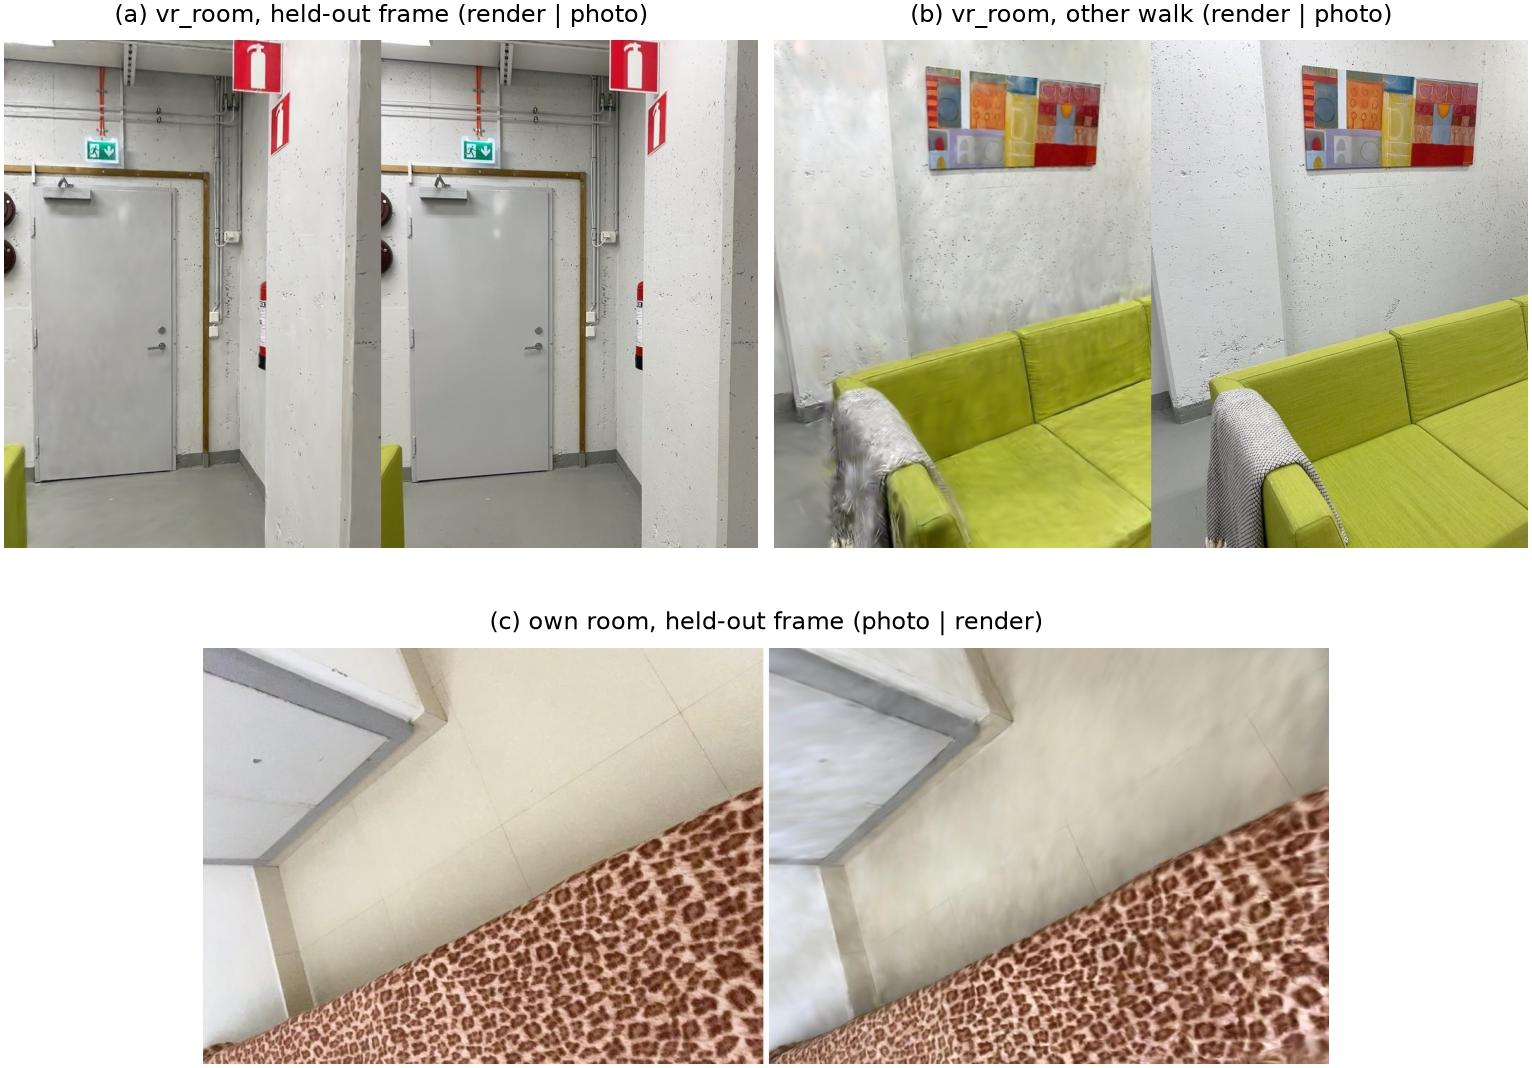
\includegraphics[width=0.9\linewidth]{figures/renders.jpg}
	\caption{Renders on held-out frames (GPU machine). (a) A held-out frame of the \texttt{vr\_room} training walk and (b) a frame of its separate walk, render left; (c) our own room, render right.}
	\label{fig:renders}
\end{figure}

\subsection{Walkability}
Both rooms were walked in the SuperSplat Viewer on the laptop (Table~\ref{tab:walk}). In \texttt{vr\_room} the walker starts inside the room at eye height, walls stop the walker at the visible surface and the floor holds; our own room was judged good by Aswin, without recording each check. In both screen recordings the overlay showed a frame time of 10.0\,ms at every sampled moment while the GPU time varied, which suggests the display, not rendering, set the frame rate. Close to a million Gaussians therefore needed no pruning, unlike the 400--500k limit of v1's browser viewer.

\begin{table}[!htb]
\caption{Walk tests (laptop, Chrome). Times are read from the viewer's overlay in the screen recordings at regular samples.}
\label{tab:walk}
\centering
\small
\begin{tabular}{lccccc}
\hline
\textbf{Room} & \textbf{Gaussians} & \textbf{Spawn inside} & \textbf{Walls stop, floor holds} & \textbf{Frame} & \textbf{GPU} \\
\hline
\texttt{vr\_room} & 908k & yes & yes & 10.0\,ms & 2.5--8.3\,ms \\
Own room & 746k & \multicolumn{2}{c}{judged good (not itemised)} & 10.0\,ms & 2.9--7.1\,ms \\
\hline
\end{tabular}
\end{table}

\subsection{Walk-collision accuracy}
\label{sec:collision-results}
Table~\ref{tab:collision} and Figure~\ref{fig:collision} give the collision study. The default collision from the splat (S) has gaps at body height, along one wall and at furniture, so the walkable area leaks out of the room (11.3\,m$^2$ against the scan's 6.5\,m$^2$): IoU 0.58, with 17.8\% of the walls the phone saw missing. Collision from DN-Splatter's mesh (M) follows the scan closely: IoU 0.81, 1.7\% missed, and a 95th-percentile offset of 10 instead of 20\,cm, but with 0.04\,m$^2$ of phantom obstacles (16 cells of 5\,cm) where S has none. M therefore passes P1, P3 and P4 (the median offset ties at 0 at this resolution) and fails P2, so the all-four rule we set is not met. Raw phone LiDAR (L) is unusable for collision (IoU 0.06, 4.3\,m$^2$ of phantom obstacles from noise and stray points), so the training step that filters the depth matters. Polycam's mesh (P), aligned in its best case, is almost as good as M but with more phantom obstacles.

\begin{table}[!htb]
\caption{Walk-collision accuracy against the laser scan of \texttt{vr\_room} (laptop). All sources use the same splat-transform pipeline; measured on a 5\,cm grid between 0.2 and 1.8\,m above the floor.}
\label{tab:collision}
\centering
\small
\begin{tabular}{lccccc}
\hline
\textbf{Source} & \textbf{IoU $\uparrow$} & \textbf{Phantom $\downarrow$} & \textbf{Missed $\downarrow$} & \textbf{Offset med./p95} & \textbf{Walkable} \\
\hline
S: splat (default) & 0.577 & \textbf{0.00}\,m$^2$ & 17.8\% & 0 / 20\,cm & 11.3\,m$^2$ \\
M: DN-Splatter mesh & \textbf{0.809} & 0.04\,m$^2$ & \textbf{1.7\%} & 0 / \textbf{10}\,cm & 7.6\,m$^2$ \\
P: Polycam mesh & 0.794 & 0.22\,m$^2$ & 1.8\% & 0 / 10\,cm & 6.9\,m$^2$ \\
L: raw phone LiDAR & 0.059 & 4.27\,m$^2$ & 47.0\% & 5 / 41\,cm & 11.4\,m$^2$ \\
GT: laser scan & 1 & 0 & 0\% & 0 / 0\,cm & 6.5\,m$^2$ \\
\hline
\end{tabular}
\end{table}

\begin{figure}[!htb]
	\centering
	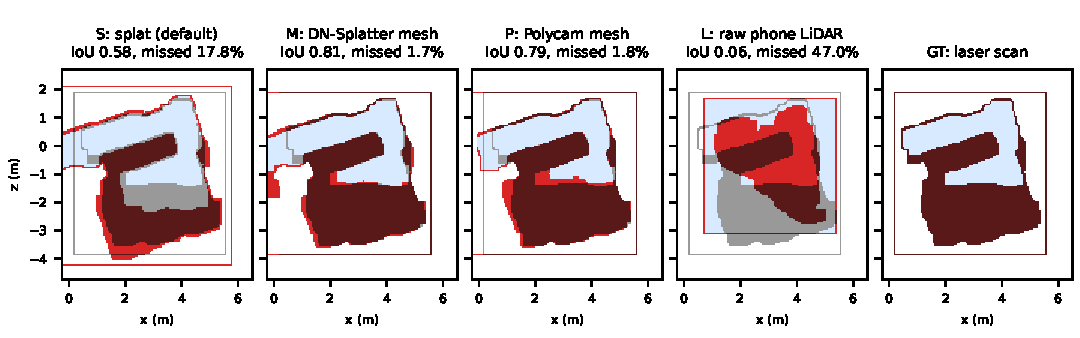
\includegraphics[width=\linewidth]{figures/collision.pdf}
	\caption{Floor plans of the \texttt{vr\_room} walk collision at body height. Red: the source's collision; grey: the laser scan's; dark red: both; light blue: walkable from the spawn. The outer rectangles close each collision volume's bounding box.}
	\label{fig:collision}
\end{figure}

The difference was not felt in practice: walking both versions freely, Aswin noticed no difference between S and M. The gaps lie at furniture and wall stretches that a free walk did not reach. The study has clear limits: one room (the only one of ours with a laser scan); the reference is the scan's own collision through the same 5\,cm pipeline; the 5\,cm cells make the median offset coarse; and S uses the real Gaussians while M, L, P and GT were converted into 2\,cm splats, which may itself contribute to the difference.

\subsection{Negative results: capture check and tracking repair}
\label{sec:negative}
\label{sec:capcheck}
\textbf{Capture check.} Its verdicts matched what we knew: \texttt{cap3} was flagged as broken tracking (Figure~\ref{fig:capcheck}, left), and \texttt{cap1}, \texttt{cap2} and \texttt{vr\_room} were asked to recapture some areas but not flagged as broken; it ran in 18--52\,s per room on the laptop. Its pre-agreed validation, comparing labels with the trained model's error on held-out frames, failed both criteria (Table~\ref{tab:capcheck}). Under-covered patches had only slightly higher error than OK patches, with overlapping intervals, and textureless patches had \emph{lower} error. Coverage predicted the worst 20\% of patches no better than chance (AUC 0.53--0.54), and texture added 0.046 AUC, short of the 0.05 required. A likely reason, found afterwards, is that a per-pixel colour error rewards smooth renders of plain walls: with 1$-$SSIM as the error (not pre-agreed), texture separated bad patches with an AUC of 0.73--0.82, in the direction ``more detail, more error''. The check is kept as a fallback, not claimed as a result.

\begin{table}[!htb]
\caption{Capture-check validation (laptop): mean held-out patch error (absolute colour error, 0--1) with bootstrap 95\% intervals. The criterion required under-covered and textureless patches to exceed OK patches with non-overlapping intervals in the test room.}
\label{tab:capcheck}
\centering
\small
\begin{tabular}{lccc}
\hline
\textbf{Room} & \textbf{OK} & \textbf{Under-covered} & \textbf{Textureless} \\
\hline
\texttt{vr\_room} (calibration) & 0.033 [0.029, 0.036] & 0.036 [0.033, 0.039] & 0.016 [0.010, 0.022] \\
\texttt{cap2} (test) & 0.056 [0.049, 0.065] & 0.063 [0.053, 0.074] & 0.034 [0.020, 0.057] \\
\hline
\end{tabular}
\end{table}

\begin{figure}[!htb]
	\centering
	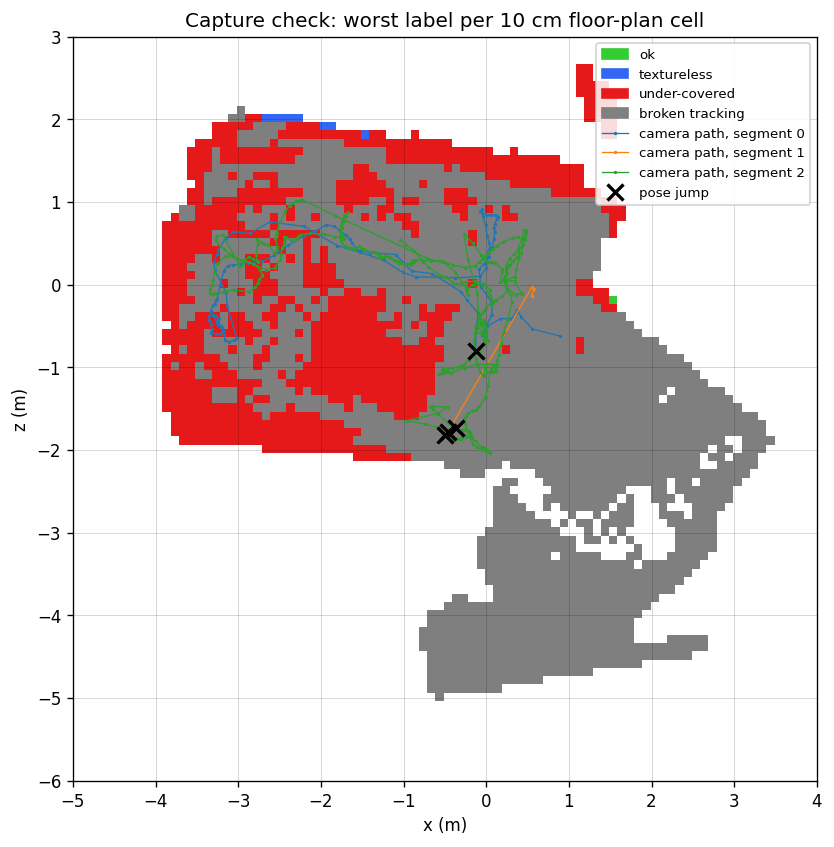
\includegraphics[height=5.6cm]{figures/capcheck_cap3.png}\hfill
	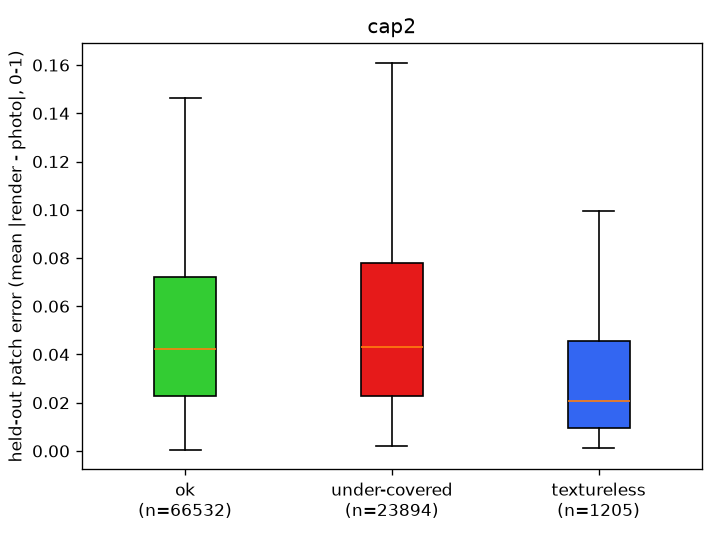
\includegraphics[height=5.6cm]{figures/capcheck_error_cap2.png}
	\caption{Capture check. Left: top-down map of \texttt{cap3}, worst label per 10\,cm cell, with the camera path coloured by tracking segment and pose jumps marked; grey areas were seen only by frames with broken tracking. Right: held-out patch error by label in the test room; textureless patches have lower error, against the check's claim.}
	\label{fig:capcheck}
\end{figure}

\textbf{Tracking repair.} The second attempt registered \texttt{cap3}'s separate sweeps to each other before training. The registration worked (fitness 0.87, turn $-0.9^\circ$, tilt $0.6^\circ$), but there was nothing to repair: before any repair the first sweep's depth already lay within 2.4\,cm of the main sweep with Polycam's corrected poses (2.7\,cm with ARKit's), close to the main sweep's 1.9\,cm agreement with itself. ARKit had relocalised, and only seven transition frames (118--124) carried the 2\,m jumps. The pre-agreed premise was false, and the added surface (4.7\%) fell below the required 5\%.

\subsection{Comparison with existing implementations}
Table~\ref{tab:compare} compares existing ways to obtain the model or its walk collision with our pipeline, all run and measured by us on \texttt{vr\_room}. Plain splats render the training walk best but give the least accurate geometry; the viewer's default collision from the splat leaks out of the room; raw phone LiDAR cannot be used for collision; and Polycam's mesh gives collision almost as good as ours, with more phantom obstacles (we did not evaluate the app's other outputs). Our combination, DN-Splatter's splat for viewing and its mesh for collision, has the most accurate geometry and the best collision on every measure except phantom obstacles.

\begin{table}[!htb]
\caption{Comparison of existing implementations with ours on \texttt{vr\_room} (our measurements; ``--'': not applicable or not measured).}
\label{tab:compare}
\centering
\begin{adjustbox}{max width=\linewidth}
\begin{tabular}{L{5.2cm}cccccc}
\hline
\textbf{Method (implementation)} & \textbf{PSNR within / with} & \textbf{Mesh acc.} & \textbf{F@5\,cm} & \textbf{Walk IoU} & \textbf{Phantom} & \textbf{Missed} \\
\hline
Plain 3DGS splats \cite{kerbl3dgs} (nerfstudio, priors off) & \textbf{26.84} / 23.24\,dB & 5.85\,cm & 0.638 & -- & -- & -- \\
SuperSplat default: collision from the splat \cite{splattransform} & same splat as ours & -- & -- & 0.577 & \textbf{0.00}\,m$^2$ & 17.8\% \\
Raw phone LiDAR, no reconstruction & -- & -- & -- & 0.059 & 4.27\,m$^2$ & 47.0\% \\
Polycam app mesh \cite{polycam} & -- & -- & -- & 0.794 & 0.22\,m$^2$ & 1.8\% \\
\textbf{Ours}: DN-Splatter splat + mesh collision & 26.32 / \textbf{23.50}\,dB & \textbf{1.76\,cm} & \textbf{0.926} & \textbf{0.809} & 0.04\,m$^2$ & \textbf{1.7\%} \\
\hline
\end{tabular}
\end{adjustbox}
\end{table}

\section{Conclusion and future scope}
\label{sec:conclusion}

RoomRecon turns an iPhone capture of a room into a photoreal Gaussian splat that can be walked through with collision, using maintained tools for almost every stage and our own code for the glue and the evaluation. Taking poses and depth from the phone, instead of estimating poses from images as in our first attempt, removed the failure on plain walls, and DN-Splatter's priors made the geometry 3.3 times more accurate than plain splats (1.76 vs 5.85\,cm from the laser scan) for 0.5\,dB less PSNR near the training walk. A public room and our own room were both walkable on a 6\,GB laptop GPU. Our main measurement shows that walk collision built from DN-Splatter's mesh matches a laser scan far better than the default collision built from the splat: the walkable-area IoU rose from 0.58 to 0.81 and missed walls fell from 17.8\% to 1.7\%, at the cost of 0.04\,m$^2$ of phantom obstacles, which failed one of our four pre-agreed criteria. Polycam's mesh of the same capture performed almost as well, both as collision (0.79, 1.8\%) and as geometry (1.86\,cm from the scan), so the main gain is over the default splat collision, not over existing apps. The gap was not felt in a free walk and the study covers one room, so we present it as a measured difference, not a general law. Two other novelty attempts, a capture check and a tracking repair, failed the tests we set in advance; we report them because they show what did not work and why.

Two directions follow from this work:
\begin{enumerate}
\item \textbf{Repeat the collision study on more rooms.} MuSHRoom provides reference meshes for all ten of its rooms, which would show whether the advantage of mesh-based collision holds beyond \texttt{vr\_room} and whether the mesh should become the default collision source.
\item \textbf{Poses from images for phones without LiDAR.} Feed-forward models such as VGGT \cite{wang2025vggt} and MASt3R-SfM \cite{duisterhof2025mast3rsfm} could be tested on the plain-walled bedroom that defeated our v1.
\end{enumerate}

\section*{Acknowledgements}
We thank IIIT Kottayam for access to its GPU server, and Kaggle for free GPU sessions. We used the MuSHRoom dataset \cite{ren2024mushroom} (CC BY 4.0) and, in v1, Apple's ARKitScenes \cite{baruch2021arkitscenes}. Our pipeline is built on open-source work by others: nerfstudio \cite{tancik2023nerfstudio}, DN-Splatter \cite{turkulainen2025dnsplatter, dnsplattercode}, gsplat \cite{ye2025gsplat}, Omnidata \cite{eftekhar2021omnidata}, Open3D \cite{zhou2018open3d}, PlayCanvas' splat-transform \cite{splattransform} and SuperSplat Viewer \cite{supersplatviewer}, and pixi \cite{pixi}; captures were made with Polycam \cite{polycam}. In v1 we also used COLMAP \cite{schoenberger2016colmap}, hloc \cite{sarlin2019hloc} with SuperPoint \cite{detone2018superpoint} and LightGlue \cite{lindenberger2023lightglue}, ORB-SLAM3 \cite{campos2021orbslam3}, GaussianSplats3D \cite{gaussiansplats3d} and NeRFCapture \cite{nerfcapture}.


\bibliography{refs}

\end{document}
